\chapter{Introduzione}
Nell'era dell'information Overload, dove giornalmente si producono quantità considerevoli di dati, memorizzati su opportuni database aziendali e non, potrebbe risultare utile utilizzare degli strumenti in grado produrre automaticamente della conoscenza a partire da questa mole di dati. Una metodologia propensa a fare ciò, è la metodologia KDD (\emph{Knowledge Discovery Databases}). 
La prima definizione da attribuire a questa metodologia è stata quella di:

\emph{Intero \textbf{processo} di estrazione di conoscenza, dalla raccolta e pre-processing dei dati, fino alla interpretazione dei risultati"\cite{DBLP:conf/kdd/1995}}


Successivamente Fayyad et al.,hanno raffinato tale definizione trasformandola in: 

\emph{Knowledge discovery is the nontrivial extraction of implicit, previously unknown, and potentially useful information from data.}
\cite{citeulike:1550195} Definendo quindi il processo KDD come un processo in grado di estrarre dai dati delle informazioni non banali, sconosciute e potenzialmente utili. Il processo KDD si articola in diverse fasi cosi come mostrato in figura \ref{kddprocess}.

\begin{figure}[hbtp]
\centering
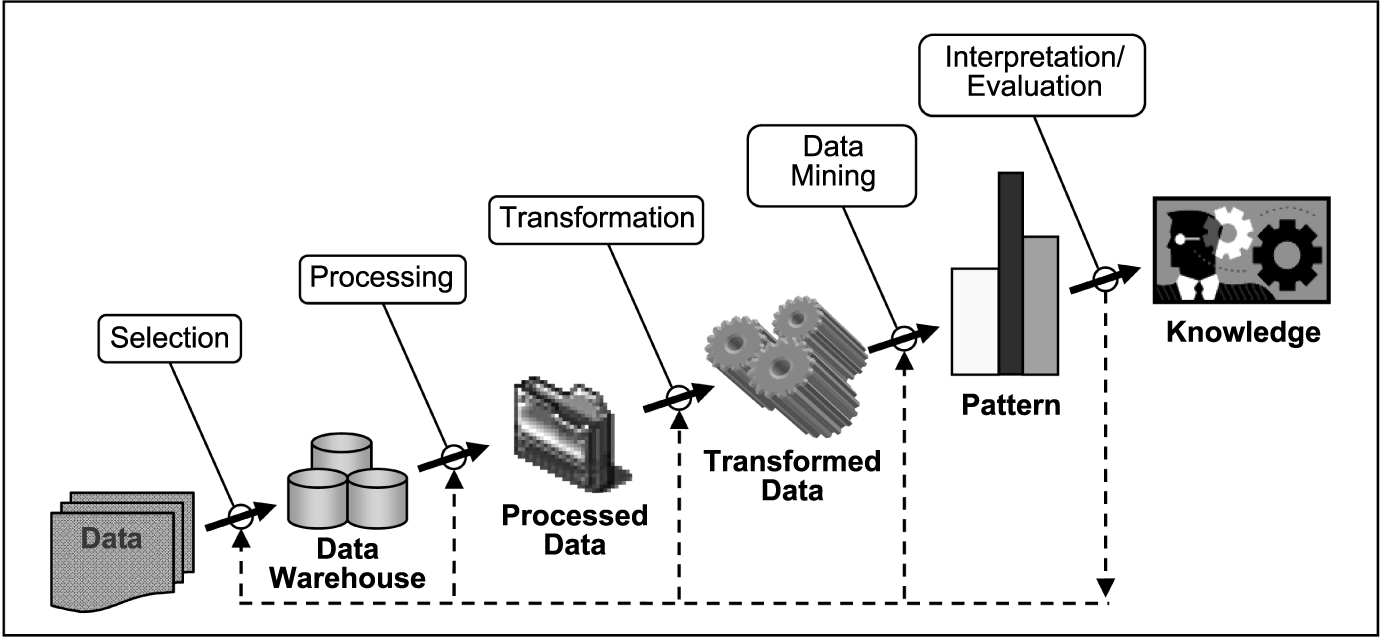
\includegraphics[width=0.8\textwidth]{./images/kddprocess.png}
\caption{Processo KDD}
\label{kddprocess}
\end{figure}

Il Data mining rappresenta la fase principale del processo KDD, il cui compito può consistere o nell'adattare un modello esistente ai dati a disposizione, oppure nel determinare dei possibili pattern ricorrenti tra i dati osservati utilizzando o delle tecniche di machine learning oppure delle tecniche statistiche. 

\section{CRISP-DM}
Per l'applicazione del processo di KDD si seguirà il modello del CRISP-DM (\emph{\textbf{CR}oss \textbf{I}ndustry \textbf{S}tandard \textbf{P}rocess for \textbf{D}ata \textbf{M}ining})
\cite{wirth2000crisp}
, in quanto, tale modello, risulta essere lo standard riconosciuto a livello industriale per la conduzione dei processi di KDD.
Il CRISP-DM si compone di sei fasi il cui ordine non è prestabilito in modo vincolante ma può variare da applicazione ad applicazione. Tipicamente le fasi di cui si compone il modello, vengono eseguite come mostrato in figura \ref{CRISPDM}.

\begin{figure}[hbtp]
\centering
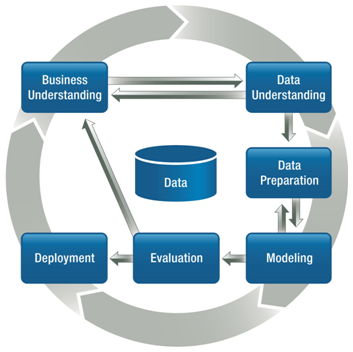
\includegraphics[width=0.5\textwidth]{./images/CRISPDM.png}
\caption{CRISP-DM}
\label{CRISPDM}
\end{figure}

Di seguito verranno esaminate le singole fasi in maniera più approfondita e per ognuna di essa, verrà illustrato l'utilizzo fatto all'interno del contesto del progetto preso in esame.